\documentclass[12pt]{article}
\usepackage[utf8]{inputenc}
\usepackage{hyperref}
\usepackage{color}
\usepackage{csquotes}
\usepackage{fullpage}
\usepackage{tikz}
\usetikzlibrary{matrix}
\usepackage{amsmath}


\title{CSCI1410, Fall 2018 ~\\
Assignment 5: Reinforcement Learning}
\date{Code Due Monday, November 5 ~\\
Writeup Due Thursday, November 8}
\author{ }

\setlength{\parindent}{0pt}
\setlength{\parskip}{1ex}
\usepackage{color}
\begin{document}

\maketitle


\section{Introduction}
After weeks of a broken phone screen, George has finally decided to drive himself to the Apple store to get it fixed. Unfortunately, his car is now a driverless, self-learning machine! George and his iPhone are now at the mercy of how well his autonomous car can make decisions. Your job is to implement reinforcement learning algorithms so his car can make it to the Apple store and get his phone fixed!

This assignment has three parts:
\begin{enumerate}
    \item In the first part you will implement tabular SARSA and SARSA lambda to help navigate a taxi to its destination. 
    \item In the second part you will implement SARSA lambda with Fourier basis functions to help a car stuck in a deep valley.
    \item In the third part, you will answer written questions about reinforcement learning.
\end{enumerate}
The coding portions use OpenAI Gym, an open source library giving access to different problem domains. The installation instructions for Gym are present in detail in Section~\ref{gym_install}.

\section{Taxi: SARSA and SARSA lambda}
\par {In this problem, your goal is to help George get to a depot. It is important to remember that the learner's only perception of the world is 1) an index for the current state of the world and, and 2) an index for the action it takes. Further, the taxi has no clue of the reward function it is trying to optimize. Your job is to help the taxi learn a policy that maximizes rewards by interacting with its environment. You will implement the SARSA and SARSA-lambda algorithms.
}

The domain itself is a $5 \times 5$ grid world, with a taxi and George. The taxi has the actions of moving north, south, east, or west. The taxi can pick up George and drop him off. 
A visualization of the domain can be seen in Figure~\ref{fig:taxi}. Here the taxi is the large yellow rectangle, and George is at the depot with the blue letter. Further, George's goal location is marked by a purple letter.
\begin{figure}
    \centering
    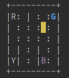
\includegraphics{taxi.png}
    \caption{A taxi problem visualization}
    \label{fig:taxi}
\end{figure}

\subsection{Stencil Code}
Here we've briefly described each file and its function. Refer to comments in the stencil for more details.

\begin{itemize}
\item \texttt{tabular\textunderscore sarsa.py}: This file is the parent class of the tabular Sarsa code that you will be implementing. There are numpy arrays: (\texttt{qtable}) for storing state-action values,  (\texttt{etable}) for storing eligibility values and  (\texttt{policy}) for storing the policy. \textbf{Do not change this file.}

\item \texttt{taxi\textunderscore sarsa.py}: Here you will implement the SARSA update rule within the \texttt{learn\textunderscore policy} function of this file. You will need to change the \texttt{qtable} array to do this. 
\begin{itemize}
\item There is a \texttt{LearningPolicy} function provided to query for actions using the state-action values we are learning. Do not edit the \texttt{LearningPolicy} function.
\item The code currently writes out the policy and state-action values to files \\ \texttt{policy\textunderscore taxi\textunderscore sarsa.npy} and \texttt{qvalues\textunderscore taxi\textunderscore sarsa.npy}, respectively.

You must submit saved versions of these files from a reasonable run for grading by renaming the saved files as \texttt{policy\textunderscore taxi\textunderscore sarsa\textunderscore grading.npy} and  \\ \texttt{qvalues\textunderscore taxi\textunderscore sarsa\textunderscore grading.npy}. We will only grade the renamed files.
The file shows an example of sampling from the gym environment and rendering the environment.
\end{itemize}

\item \texttt{taxi\textunderscore sarsa\textunderscore lambda.py}: Similar to the previous file, here you need to implement the SARSA update rule within the \texttt{learn\textunderscore policy} function of \texttt{taxi\textunderscore sarsa\textunderscore lambda.py}. You will change the \texttt{qtable} array, and the \texttt{etable} array. There is a \texttt{LearningPolicy} provided to query for actions using the state-action values we are learning. Do not edit the \texttt{LearningPolicy} function. 
\begin{itemize}
\item Again, we are writing out the policy and state-action values as \\ \texttt{policy\textunderscore taxi\textunderscore sarsa\textunderscore lambda.npy} and \texttt{qvalues\textunderscore taxi\textunderscore sarsa\textunderscore lambda.npy}, respectively. You should submit saved files from a reasonable run for grading by renaming the saved numpy arrays to  \texttt{policy\textunderscore taxi\textunderscore sarsa\textunderscore lambda\textunderscore grading.npy} and   \\ \texttt{qvalues\textunderscore taxi\textunderscore sarsa\textunderscore lambda\textunderscore grading.npy}. 
We will only grade the renamed files.
\end{itemize}
\end{itemize}

\subsection{Objective}
We want you to code Sarsa and Sarsa-lambda and plot learning curves averaged over ten runs.
You should submit the two learning curve plots as part of your written handins.
The grading will be performed by looking at your learning curves, and auto-grading using the saved policy and Q-values.
With the learning curve please submit your learning parameters of learning rates (alphas) and lambda.

\section{Mountain-car}
In this problem a car is stuck at the bottom of a valley. It needs to get to the top of the mountain marked with a flag. 
A visualization of the domain can be seen in Figure~\ref{fig:mountain_car}. The car needs to rock back and forth repeatedly to get out of the valley, as it does not have enough power to just go up the hill. The agent state space consists of the car's position along the x-axis and its velocity. The agent's actions are to go left, go right, or do nothing.
\begin{figure}[h!]
    \centering
    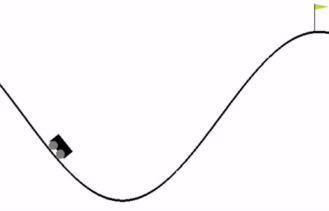
\includegraphics{mountain_car.png}
    \caption{A mountain car problem visualization}
    \label{fig:mountain_car}
\end{figure}
\subsection{Stencil Code}
The only file you should modify is \texttt{mountain\textunderscore car\textunderscore sarsa\textunderscore fourier.py}. Here we introduce the helper functions briefly, but please read the code stencil carefully to understand the functionality in more detail. \textbf{You should not modify any functions except for those you are instructed to.}
\begin{enumerate}
\item \texttt{normalize\textunderscore state}: This function normalizes states variables within range of $0$ to $1$. This needs to be done before you compute basis functions of the states. 
\item \texttt{phi}: This function takes in a normalized state and computes its features. \textbf{You need to fill in this function.}
\item \texttt{create\textunderscore multipliers}: This function creates the Fourier basis coefficients for the cosine function. \textbf{You need to fill in this function.}
\item \texttt{action\textunderscore value} and \texttt{action\textunderscore values} : These functions return Q-value for a state-action pair or Q-values for a state for all possible actions respectively. 
\item \texttt{learning\textunderscore policy} and \texttt{test\textunderscore policy} These functions return the best action for a given input state with and without exploration respectively. After an agent has learned a policy it does not need to explore hence a separate policy.
\item \texttt{SARSA\textunderscore Learning}: This function learns the weights for the QValue function using SARSA-lambda. Some of the function is filled in so you can interface to the rest of the code, but \textbf{you need to fill in the update rules.} \\ 

\item \texttt{SARSA\textunderscore Test}: This function uses the weights calculated or saved to plan over a specified number of episodes. You can use this code to test your policy's behaviour before you submit it.  
\end{enumerate}

We are saving the weights learned at the end of the learning period in  \texttt{SARSA\textunderscore Learning} as \texttt{mountain\textunderscore car\textunderscore saved\textunderscore weights.npy}. Make sure to submit a saved version of this file from a good run to  \texttt{mountain\textunderscore car\textunderscore saved\textunderscore weights\textunderscore grading.npy}.

\subsection{Objective}
We want you to code SARSA-lambda and function approximation for the mountain car scenario. The grading will be performed by auto-grading using the saved weights. You can tell if your learning policy is correct by creating a learning curve like the ones generated by the taxi problem. You do not need to submit the learning curve for Mountain Car as a part of your handin.
\newline
Tip: You can use numpy.load() to look at your saved numpy files.

\section{Written Questions}
Answer the following questions in clearly labeled sections.
\begin{enumerate}
    \item 
    \begin{enumerate}
        \item What is the fundamental difference between the probabilistic planning and reinforcement learning problems? Your answer should be one sentence.
        
        \item Discuss at least one important consequence of this difference, as it applies to solving the problems.
        
        \item Give an example of a probabilistic planning problem. Modify it slightly to create a reinforcement learning problem.
        
    \end{enumerate}
    
    \item Suppose you have a reinforcement learning agent that learns an estimate of the action-value (Q) function of its environment and then uses its estimate to choose actions. 
    
    When the agent uses its estimate of the Q-function to choose an action at state $s$, it faces a tradeoff: it can choose the action that appears to be best under its estimate, $a^* \equiv arg\max_a {Q(s, a)}$, or it can choose a different action $a_e \neq a^*$, in hopes of improving its estimate of $Q(s, a_e)$, since doing so may increase the sum of discounted reward in the long run. What is this tradeoff called, and what is one way that your agent could manage it effectively? 
    
    
    \item Consider the following game tree:
    \begin{figure}[h]
    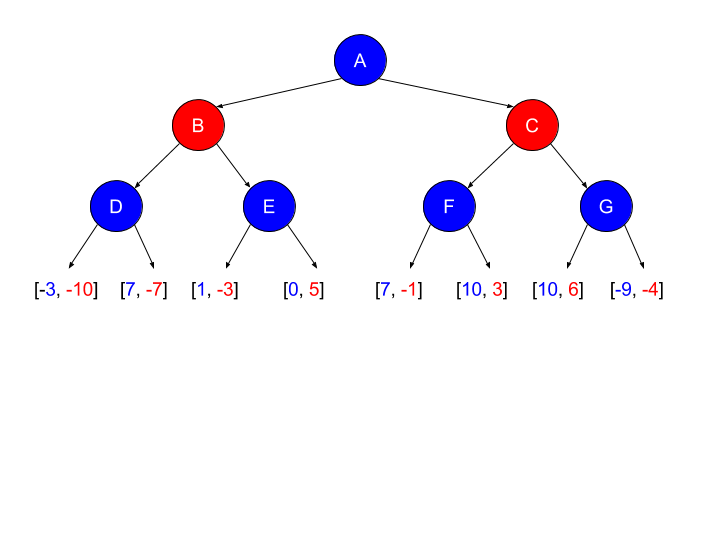
\includegraphics[scale = 0.5]{rl-game-tree.png}
    \centering
    \end{figure}
    
    The game has two players, Blue and Red.
    Blue makes decisions at blue nodes and Red makes decisions at red nodes.
    Each state of the game is represented by an upper-case letter (e.g., the top game state is `A').
    At every state, the decision-making player has two choices: \textbf{Left} or \textbf{Right}.
    The lists $[a, b]$ at the bottom of the tree represent terminal states of the game, in which Blue earns $a$ points and Red earns $b$ points. ~\\
    
    Suppose you are Blue, and you know that Red always plays the maximin action.
    How can you formulate the game as an MDP \textbf{from your perspective, such that you, as Blue, are the only decision-maker}?
    In particular, what are the set of states, the set of actions, the reward function, and the transition function?
    Solve for the action-value (Q) function, and report it in the form of a table.
    You may ignore the discount factor $\gamma$ of the MDP (or, equivalently, set it equal to 1).
\end{enumerate}
\section{Gym installation}
\label{gym_install}
There are several packages that are needed for this project. Some of the necessary packages are: \texttt{gym}, \texttt{matplotlib}, and \texttt{numpy}.
If you use the course virtual environment you shouldn't need to install anything, but if you are working locally you may need to install these by running \texttt{pip install `gym[all]'}.

\section{Grading}
Grading on questions $2.1$ and $2.2$ will be done using the policy and Q-Value numpy files submitted. The time limit for a single run is 30 seconds each. We will run these files 10 times from random start states and award full points if the average steps to completion from the random re-starts is under $30$.
You can always test the learned policy by doing the same and making sure that learned policies can complete the task in under $30$ steps when averaged over ten runs. ~\\


Grading for question $3$ is also done using an auto-grader.
The time limit for each run is 30 seconds. Here, we want to make sure that the learned policy has an average number of steps to completion under $400$ over ten runs. There is some test code provided for this question to run directly. Please read the stencil code for more details. ~\\

We will validate your implementations for correctness by looking at your learning curves, since the learning curves of the two algorithms will look different.
\textbf{If we find by looking at your code that the learning curves that you submit could not have been generated by your code, you will earn a 0 for the entire assignment.} ~\\

You can check the given \verb|rubric.txt| to see how heavily each part of the assignment weighs into your grade.

\textbf{
Note: After generating your .npy files, you need to rename them by adding `$\_$grading.npy' to the end of each file name. Incorrectly named files will not be graded.}

\section{Handin}
You should hand in your code and three saved numpy files by running \texttt{cs1410\_handin RL} from the directory containing your files.

The written problems and two learning curves should be turned on Gradescope. ~\\




\end{document}
